\documentclass[12pt, twoside]{article}
\usepackage[letterpaper, margin=1in, headsep=0.5in]{geometry}
\usepackage[english]{babel}
\usepackage[utf8]{inputenc}
\usepackage{amsmath}
\usepackage{amsfonts}
\usepackage{amssymb}
\usepackage{tikz}
\usetikzlibrary{quotes, angles}
\usepackage{graphicx}
\usepackage{enumitem}
\usepackage{multicol}

\newif\ifmeta
\metatrue %print standards and topics tags

\title{Regents Geometry}
\author{Chris Huson}
\date{September 2020}

\usepackage{fancyhdr}
\pagestyle{fancy}
\fancyhf{}
\renewcommand{\headrulewidth}{0pt} % disable the underline of the header
\raggedbottom


\fancyhead[LE]{\thepage}
\fancyhead[RO]{\thepage \\ Name: \hspace{4cm} \,\\}
\fancyhead[LO]{BECA / Dr. Huson / Geometry \\* 1-10 Solving for angle bisectors}

\begin{document}

\subsubsection*{I can solve for angle measures}
\begin{enumerate}
\item Do Now: Given $M$ bisects $\overline{PQ}$, $PM=x+7$, $PQ=23$.
\begin{multicols}{2}

  \begin{center}
    \begin{tikzpicture}
      \draw [fill, white] (0,1) circle [radius=0.05] node[below]{$P$};
      \draw [-, thick] (0,0)--(6,0);
      \draw [fill] (0,0) circle [radius=0.05] node[below]{$P$};
      \draw [fill] (3,0) circle [radius=0.05] node[below]{$M$};
      \draw [fill] (6,0) circle [radius=0.05] node[below]{$Q$};
    \end{tikzpicture}
  \end{center}
  \begin{enumerate}
    \item Mark the diagram with the values and tick marks
    \item Write an equation and solve for $x$
    \item Check your result
  \end{enumerate} 
\end{multicols} \vspace{2.5cm}


\item The ray $\overrightarrow{AD}$ bisects $\angle ABC$. $m\angle ABD=3x+1$, $m\angle DBC=5x-25$. Find $m\angle ABC$.\vspace{0.5cm}
  \begin{flushright}
    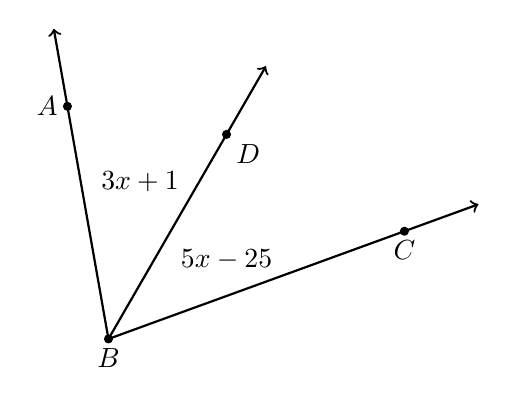
\begin{tikzpicture}
      \draw [<->, thick] (100:4)--(0,0)--(20:5);
      \draw [->, thick] (0,0)--(60:4);
      \draw [fill] (100:3) circle [radius=0.05] node[left]{$A$};
      \draw [fill] (60:3) circle [radius=0.05] node[below right]{$D$};
      \draw [fill] (0,0) circle [radius=0.05] node[below]{$B$};
      \draw [fill] (20:4) circle [radius=0.05] node[below]{$C$};
      \node at (1.5,1){$5x-25$};
      \node at (0.4,2){$3x+1$};
    \end{tikzpicture}
    \end{flushright} \vspace{1cm}

\item Two lines intersect with vertical angles $m\angle 1=2x+20$ and $m\angle 3=3x-5$. Find $m\angle 2$.
  \begin{flushleft}
  \begin{tikzpicture}[scale=0.8, rotate=30]
    \draw [<->, thick] (0,-1.5)--(10,1.5);
    \draw [<->, thick] (2,3.5)--(7,-3.5);
    \node at (1.5,1.3){$m\angle 1=2x+20$};
    \node at (7,-1){$m\angle 3=3x-5$};
    \node at (5,1){2};
    \node at (4,-1){4};
  \end{tikzpicture}
  \end{flushleft}

\newpage

\item Write the appropriate name for the type of angle depending on its measure in degrees. (acute, right, obtuse, or straight)
    \begin{enumerate}
      \item $m\angle = 90$ : \rule{4cm}{0.15mm} \bigskip
      \item $90 < m\angle < 180$ : \rule{4cm}{0.15mm} \bigskip
      \item $0< m\angle < 90$ : \rule{4cm}{0.15mm} \bigskip
      \item $m\angle = 180$ : \rule{4cm}{0.15mm} \bigskip
    \end{enumerate}

\item Write down the name of the given angle three different ways.\\
    \begin{tikzpicture}
      \draw
        (3,-1) coordinate (a) node[right] {A}
        -- (0,0) coordinate (b) node[left] {B}
        -- (2,2) coordinate (c) node[above right] {C}
        pic["1", <->, draw=black, angle eccentricity=1.2, angle radius=1cm]
        {angle=a--b--c};
    \end{tikzpicture}

\item Points that are all located on the same plane are $\rule{4cm}{0.15mm}$.

\item Spicy: Given isosceles $\triangle ABC$ with $\overline{AC} \cong \overline{BC}$. $AC=5x+7$ and $BC=3x+17$. \\ Find $AC$.\\[0.5cm]
    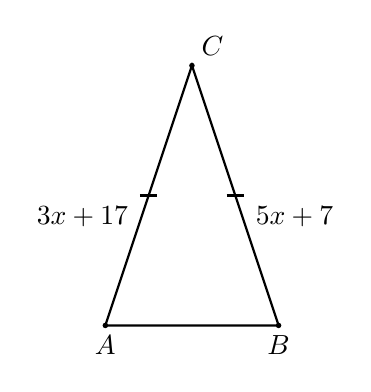
\begin{tikzpicture}[scale=0.55]
      \draw [thick](0,0)--(4,0)--(2,6)--(0,0);
      \draw [fill] (0,0) circle [radius=0.05] node[below]{$A$};
      \draw [fill] (4,0) circle [radius=0.05] node[below]{$B$};
      \draw [fill] (2,6) circle [radius=0.05] node[above right]{$C$};
      \draw [thick] (0.8,3)--(1.2,3); %tick mark
      \draw [thick] (2.8,3)--(3.2,3); %tick mark
      \node [right] at (3.25,2.5){$5x+7$};
      \node [left] at (0.75,2.5){$3x+17$};
    \end{tikzpicture}

\item Given points on the number line $E(1.2)$ and $G(5.6)$ as shown. Find the midpoint $F$ of $\overline{EG}$. Mark it on the number line and label it as an ordered pair.\\[20pt]
    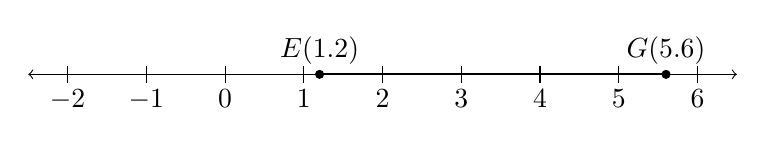
\begin{tikzpicture}
      \draw [<->] (-2.5,0)--(6.5,0);
      \foreach \x in {-2,...,6} %2 leading for diff!=1
        \draw[shift={(\x,0)},color=black] (0pt,-3pt) -- (0pt,3pt) node[below=5pt]  {$\x$};
        \draw [thick] (1.2,0)--(5.6,0);
        \draw [fill] (1.2,0) circle [radius=0.05] node[above] {$E(1.2)$};
        \draw [fill] (5.6,0) circle [radius=0.05] node[above] {$G(5.6)$};
    \end{tikzpicture}

\end{enumerate}
\end{document}